\documentclass[onecolumn, draftclsnofoot,10pt, compsoc]{IEEEtran}
\usepackage{graphicx}
\usepackage{url}
\usepackage{setspace}
\usepackage{pstricks-add}
\usepackage{float}
\usepackage{soul}
\usepackage{color}

\usepackage{listings}


% COLOR DEFINITIONS FOR CODE LISTINGS
\definecolor{codegreen}{rgb}{0,0.6,0}
\definecolor{codegray}{rgb}{0.5,0.5,0.5}
\definecolor{codepurple}{rgb}{0.58,0,0.82}
\definecolor{backcolour}{rgb}{0.95,0.95,0.92}

\lstdefinestyle{mystyle}{
    backgroundcolor=\color{backcolour},
    commentstyle=\color{codegreen},
    keywordstyle=\color{magenta},
    numberstyle=\tiny\color{codegray},
    stringstyle=\color{codepurple},
    basicstyle=\footnotesize,
    breakatwhitespace=false,
    breaklines=true,
    captionpos=b,
    keepspaces=true,
    numbers=left,
    numbersep=5pt,
    showspaces=false,
    showstringspaces=false,
    showtabs=false,
    tabsize=2
}

\lstset{
	escapeinside={(*@}{@*)},
	style=mystyle
}

\usepackage{geometry}
\geometry{textheight=9.5in, textwidth=7in}

% 1. Fill in these details
\def \CapstoneTeamName{		AKA Robotics}
\def \CapstoneTeamNumber{		13}
\def \GroupMemberOne{     Arthur Shing}
\def \GroupMemberTwo{			Kevin Talik}
\def \GroupMemberThree{   Anish Asrani}
\def \CapstoneProjectName{		How to Make an Effective Robot Comedian}
\def \CapstoneSponsorCompany{	Oregon State University}
\def \CapstoneSponsorPerson{		Heather Knight}

% 2. Uncomment the appropriate line below so that the document type works
\def \DocType{		%Problem Statement
				%Requirements Document
				%Technology Review
				Design Document
				%Progress Report
				}

\newcommand{\NameSigPair}[1]{\par
\makebox[2.75in][r]{#1} \hfil 	\makebox[3.25in]{\makebox[2.25in]{\hrulefill} \hfill		\makebox[.75in]{\hrulefill}}
\par\vspace{-12pt} \textit{\tiny\noindent
\makebox[2.75in]{} \hfil		\makebox[3.25in]{\makebox[2.25in][r]{Signature} \hfill	\makebox[.75in][r]{Date}}}}
% 3. If the document is not to be signed, uncomment the RENEWcommand below
\renewcommand{\NameSigPair}[1]{#1}

%%%%%%%%%%%%%%%%%%%%%%%%%%%%%%%%%%%%%%%
\begin{document}

\bstctlcite{IEEEexample:BSTcontrol}
\begin{titlepage}
    \pagenumbering{gobble}
    \begin{singlespace}
        \hfill
        % 4. If you have a logo, use this includegraphics command to put it on the coversheet.
        %\includegraphics[height=4cm]{CompanyLogo}
        \par\vspace{.2in}
        \centering
        \scshape{
            \huge CS Capstone \DocType \par
            {\large\today}\par
            \vspace{.5in}
            \textbf{\Huge\CapstoneProjectName}\par
            \vfill
            {\large Prepared for}\par
            \Huge \CapstoneSponsorCompany\par
            \vspace{5pt}
            {\Large\NameSigPair{\CapstoneSponsorPerson}\par}
            {\large Prepared by }\par
            Group\CapstoneTeamNumber\par
            % 5. comment out the line below this one if you do not wish to name your team
            \CapstoneTeamName\par
            \vspace{5pt}
            {\Large
                \NameSigPair{\GroupMemberOne}\par
                \NameSigPair{\GroupMemberTwo}\par
                \NameSigPair{\GroupMemberThree}\par
            }
            \vspace{20pt}
        }
        \begin{abstract}
          To make an Effective Robot Comedian, we have developed three research questions to investigate our approach to designing this system: Adapting to audience response to humor, incorporating the crowd into the performance, and the effect of characterization in anthropomorphizing the robot. This paper outlines how our research questions will be incorporated into a system, and how we will study the shared space between a robot and an audience.


        \end{abstract}
    \end{singlespace}
\end{titlepage}
\newpage
\pagenumbering{arabic}
\tableofcontents
% 7. uncomment this (if applicable). Consider adding a page break.
%\listoffigures
%\listoftables
\clearpage

% 8. now you write!
\section{Introduction}

  Comedy can come from robots of any kind. A carpet cleaning bot could miscalculate the end of a floor and tumble down a flight of stairs, or a voice-assisted tool might accidentally confuse a \textit{Dinnertime Jazz} playlist for \textit{Death Metal Essentials}. These actions that happen around a human can become shared experiences and references for the observer. For every shared task between a robot and a human, the human will often feel more empathetic towards a robot that makes an effort to be more aware of surroundings\cite{DesignExBeh:2017}. If the robot wants to become an effective comedian, it will have to attempt to be empathetic as well; it has to listen to the response of a completed action, and consider the change the bot brought to the setting.

\subsection{Scope}
This paper covers the research questions that will guide the investigation of the interaction between a crowd and
a comedian robot, as well as the main design goals for implementing comedy behaviors on a NAO Robot. There
are three areas of intended research. These areas include the development of the intelligent adaptions to the crowd
(”adaptation”), the integration of an audience into the performance of a set (”crowdwork”), and the exploration of
robotic versus humanlike storytelling, movement, and reaction to the audience (”character”). All of these components
will culminate into the robot comedian, Ginger. At the end of the academic year, we will have a Robot Comedian that we
have evaluated the effectiveness of. The main end-product is software for the variable stand-up comedy sets performed
by the NAO robot, and the analysis of audience responses to our manipulations in audience adaptation, crowdwork,
and robot or humanlike character. Both of these will be described in our final paper.


  \subsection{Purpose}
	The purpose of this document is to describe the development of the robot comedian, which involves: (1) the three
main research questions, (2) the robot behavior implementations, and (3) the experiments we plan to use to answer the
research questions.

\subsection{Intended Audience}
	This document is intended for stakeholders and developers in the research project \textit{How to Make an Effective Robot Comedian}.

	% The first section covers the adaptation algorithm, the components of a stand-up set, and audience response comprehension. The next section explains "crowd-work", and how we will examine the influence of incorporating the audience into the robot's performance. Finally, the last section will cover the diversity of being a robot comedian, and how the qualities of a robot characterize the comedian.

\section{Research Design Overview}
This section will cover the research questions for evaluating the effectiveness of a robot comedian. These questions will
be the basis of the implementation of the comedian system. All three research questions will be presented including
software requirements needed to answer the questions, and the experimental methods that will generate quantitative
data about what impacts audience experience, participation, and reactions.
The comedian system that is implemented will test three critical areas of a comedic performance corresponding
to our research. The first question is about \textbf{adaptation} of a performance – how the robot and interpret an audience
response. The second question studies \textbf{crowd work} during a show, and the choices a Comedian can make to engage the
audience. Lastly, the third considers the implications of a perceivable \textbf{character} that the robot can portray, in particular robotic versus humanlike.


\subsection{Adaptation}
\subsubsection{Goal}
We hypothesize that audiences will prefer a robot that acknowledges them, and integrates their data and responses into
its set. To test this hypothesis we propose two tests: (1) to transition to topics dependent on the audience response,
and (2) to present a crowd report upon completion of the set. The goal of this portion of the project is to determine
if incorporating the audience into the set will enhance the overall performance of the comedian. To evaluate these
hypotheses, we will conduct live studies in which people experience different versions of the software described below.
\subsubsection{Methods}
Generally, the performance will have two to three parts: the Seed Jokes, the Middle Content, and the Close. The Seed
will influence the Middle Content (which will be chosen themed jokes and basis of the show). The Middle Content will
transition to a intelligent or generalized Closing Joke when it is time to end the show.


Figure \ref{fig:joke} depicts how a joke will be represented by the robot. It will perform the joke, collect audience feedback
information, and branch to the joke that will best fit the response. At the end of the set, the robot will present a summary
of what it thought that audience liked.
\begin{figure}[H]
  \centering
  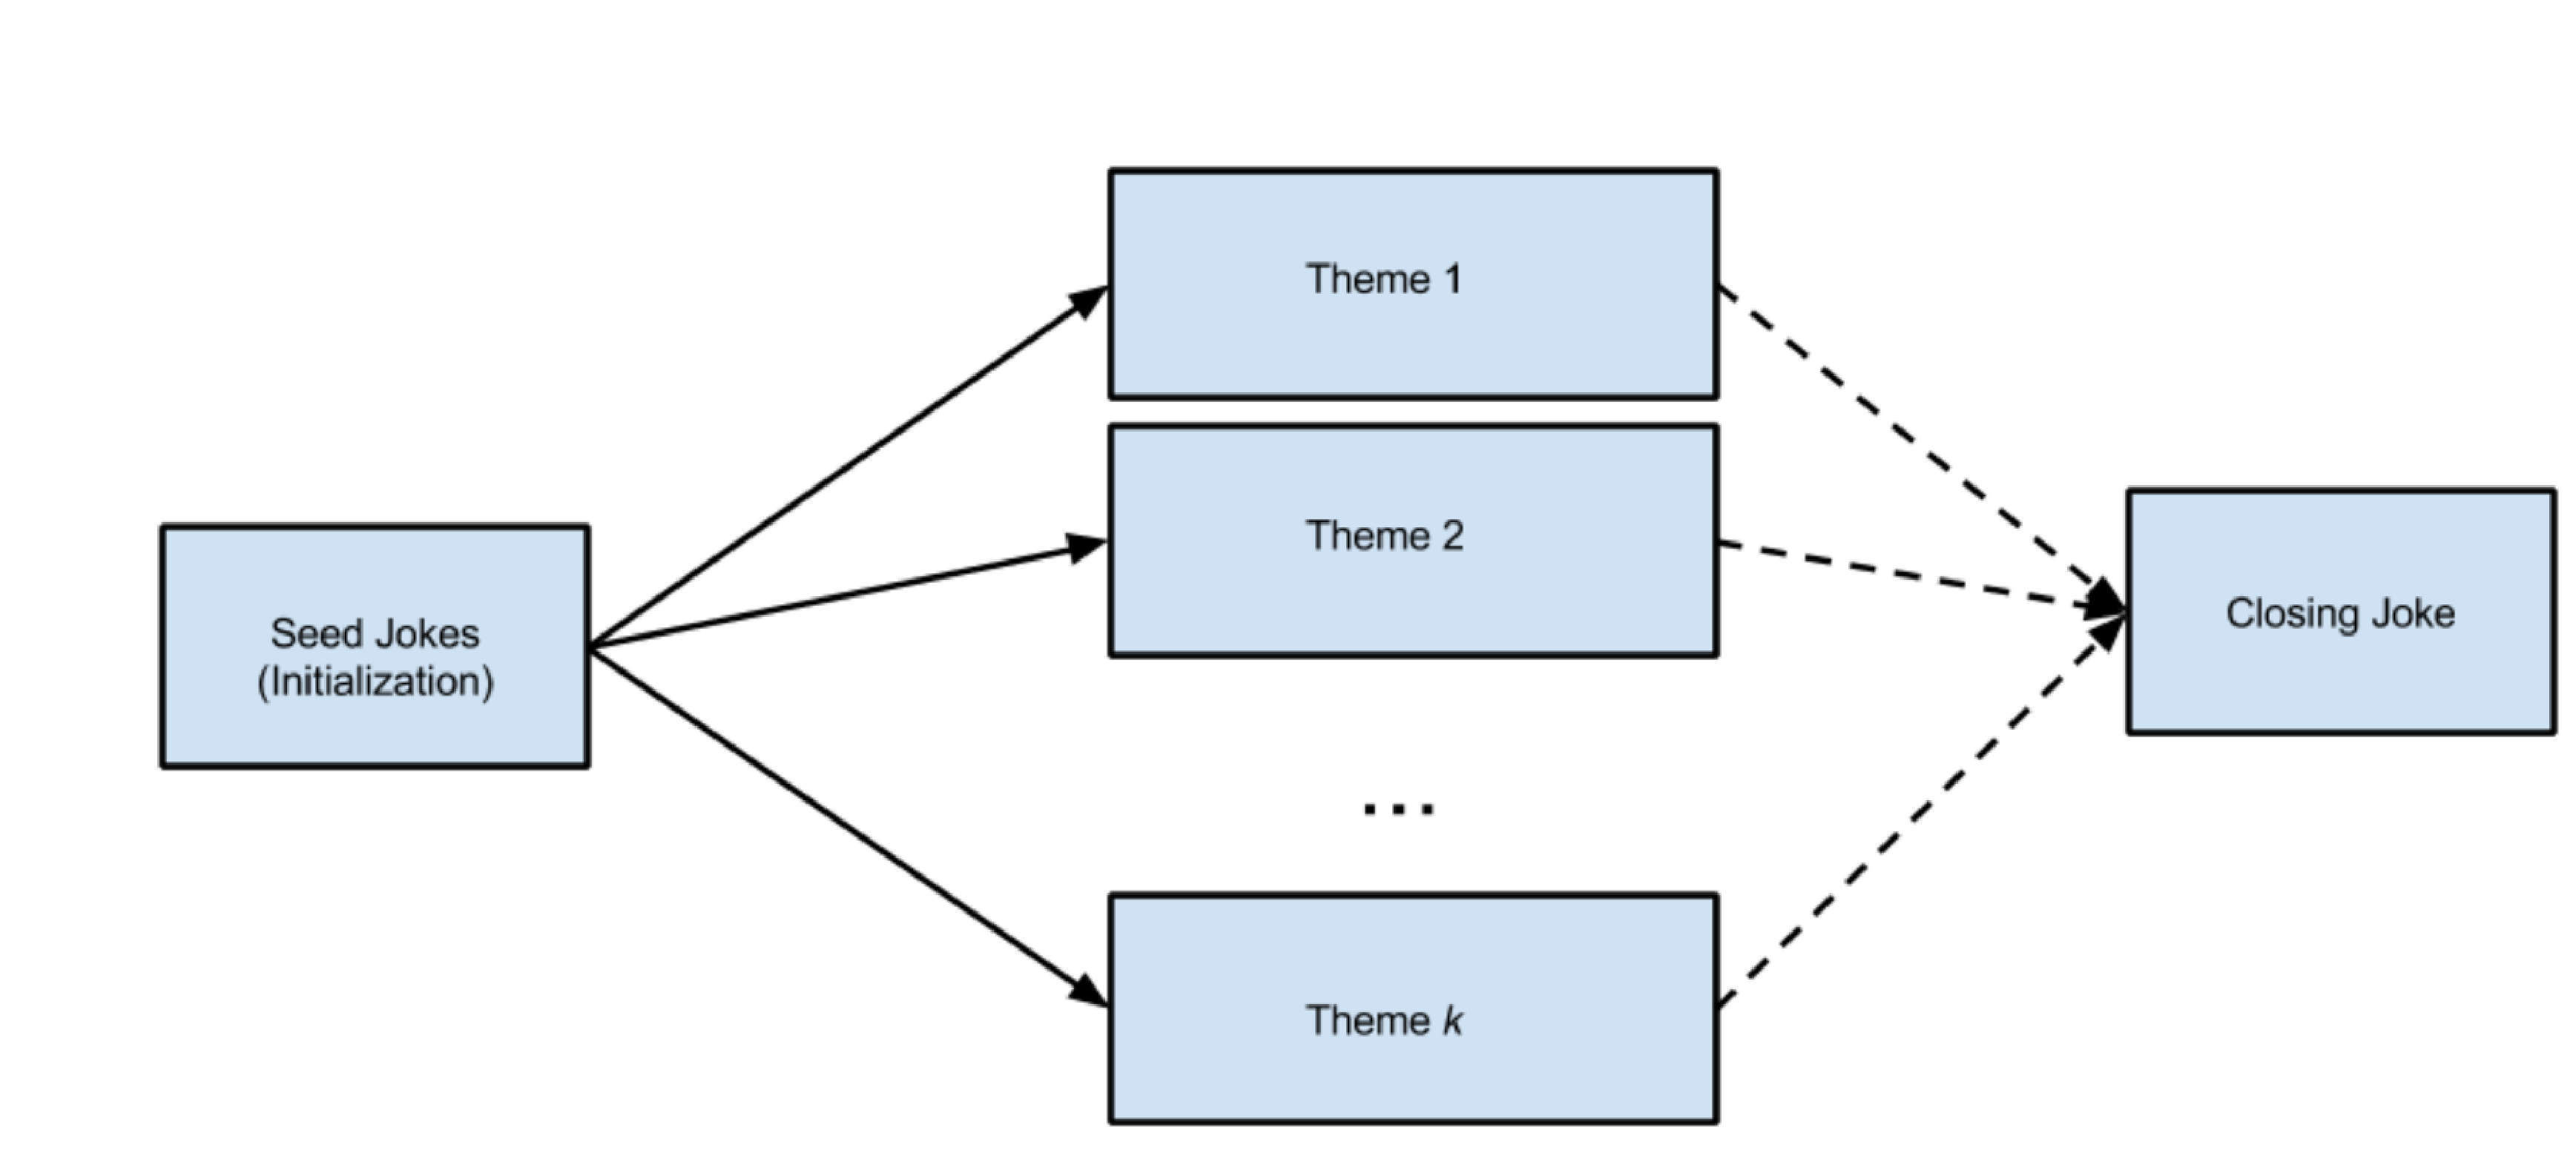
\includegraphics[width=0.75\textwidth,height=0.75\textheight,keepaspectratio]{fig0}
  \caption{This shows how the algorithm will have up to \textit{k} Themes to choose from, determined from the seed joke. The closing joke is a subset of the set of all jokes, and may be outside of a specific theme. There could be different spanning trees of jokes that end at the same closing joke}
  \label{fig:joke}
\end{figure}

In the beginning of the set, the comedian will present an ”initialization” procedure, known
as the ”Seed Jokes” to test the response of the audience to different jokes. Depending on their response, the comedian
will transition to a theme that is evaluated to be the best fit. The robot comedian will have many jokes to choose from
that contain different material, but not all audiences will like all of the jokes. Figure \ref{fig:process} shows how the theme will be
chosen from a set of up to k themes. From the Seed Jokes, one of the themes will be chosen. If there is time, we may also
explore the choice of strategic closing jokes. These jokes might be stronger jokes than some of the others, and is helpful
in ending the show on a stronger note.

For example, if two of the seed jokes are about ”food” and ”Mindfulness”, the performance will branch to the
respective theme that matches the audience response (Branch 1 ”Food” or Branch 2 ”Mindfulness”). If jokes with a
theme of ”food” are not landing with the audience, the algorithm will need to know when to transition to a new theme, or when to end the set. When the robot tells a joke, it needs to be able to analyze the feedback and choose the next joke
to perform. This needs to be done quickly, so that the robot is not spending noticeable time (for the audience) choosing
a joke. There may not be a lot of jokes to choose from, but the choice needs to be made fast.

\begin{figure}[H]
  \centering
  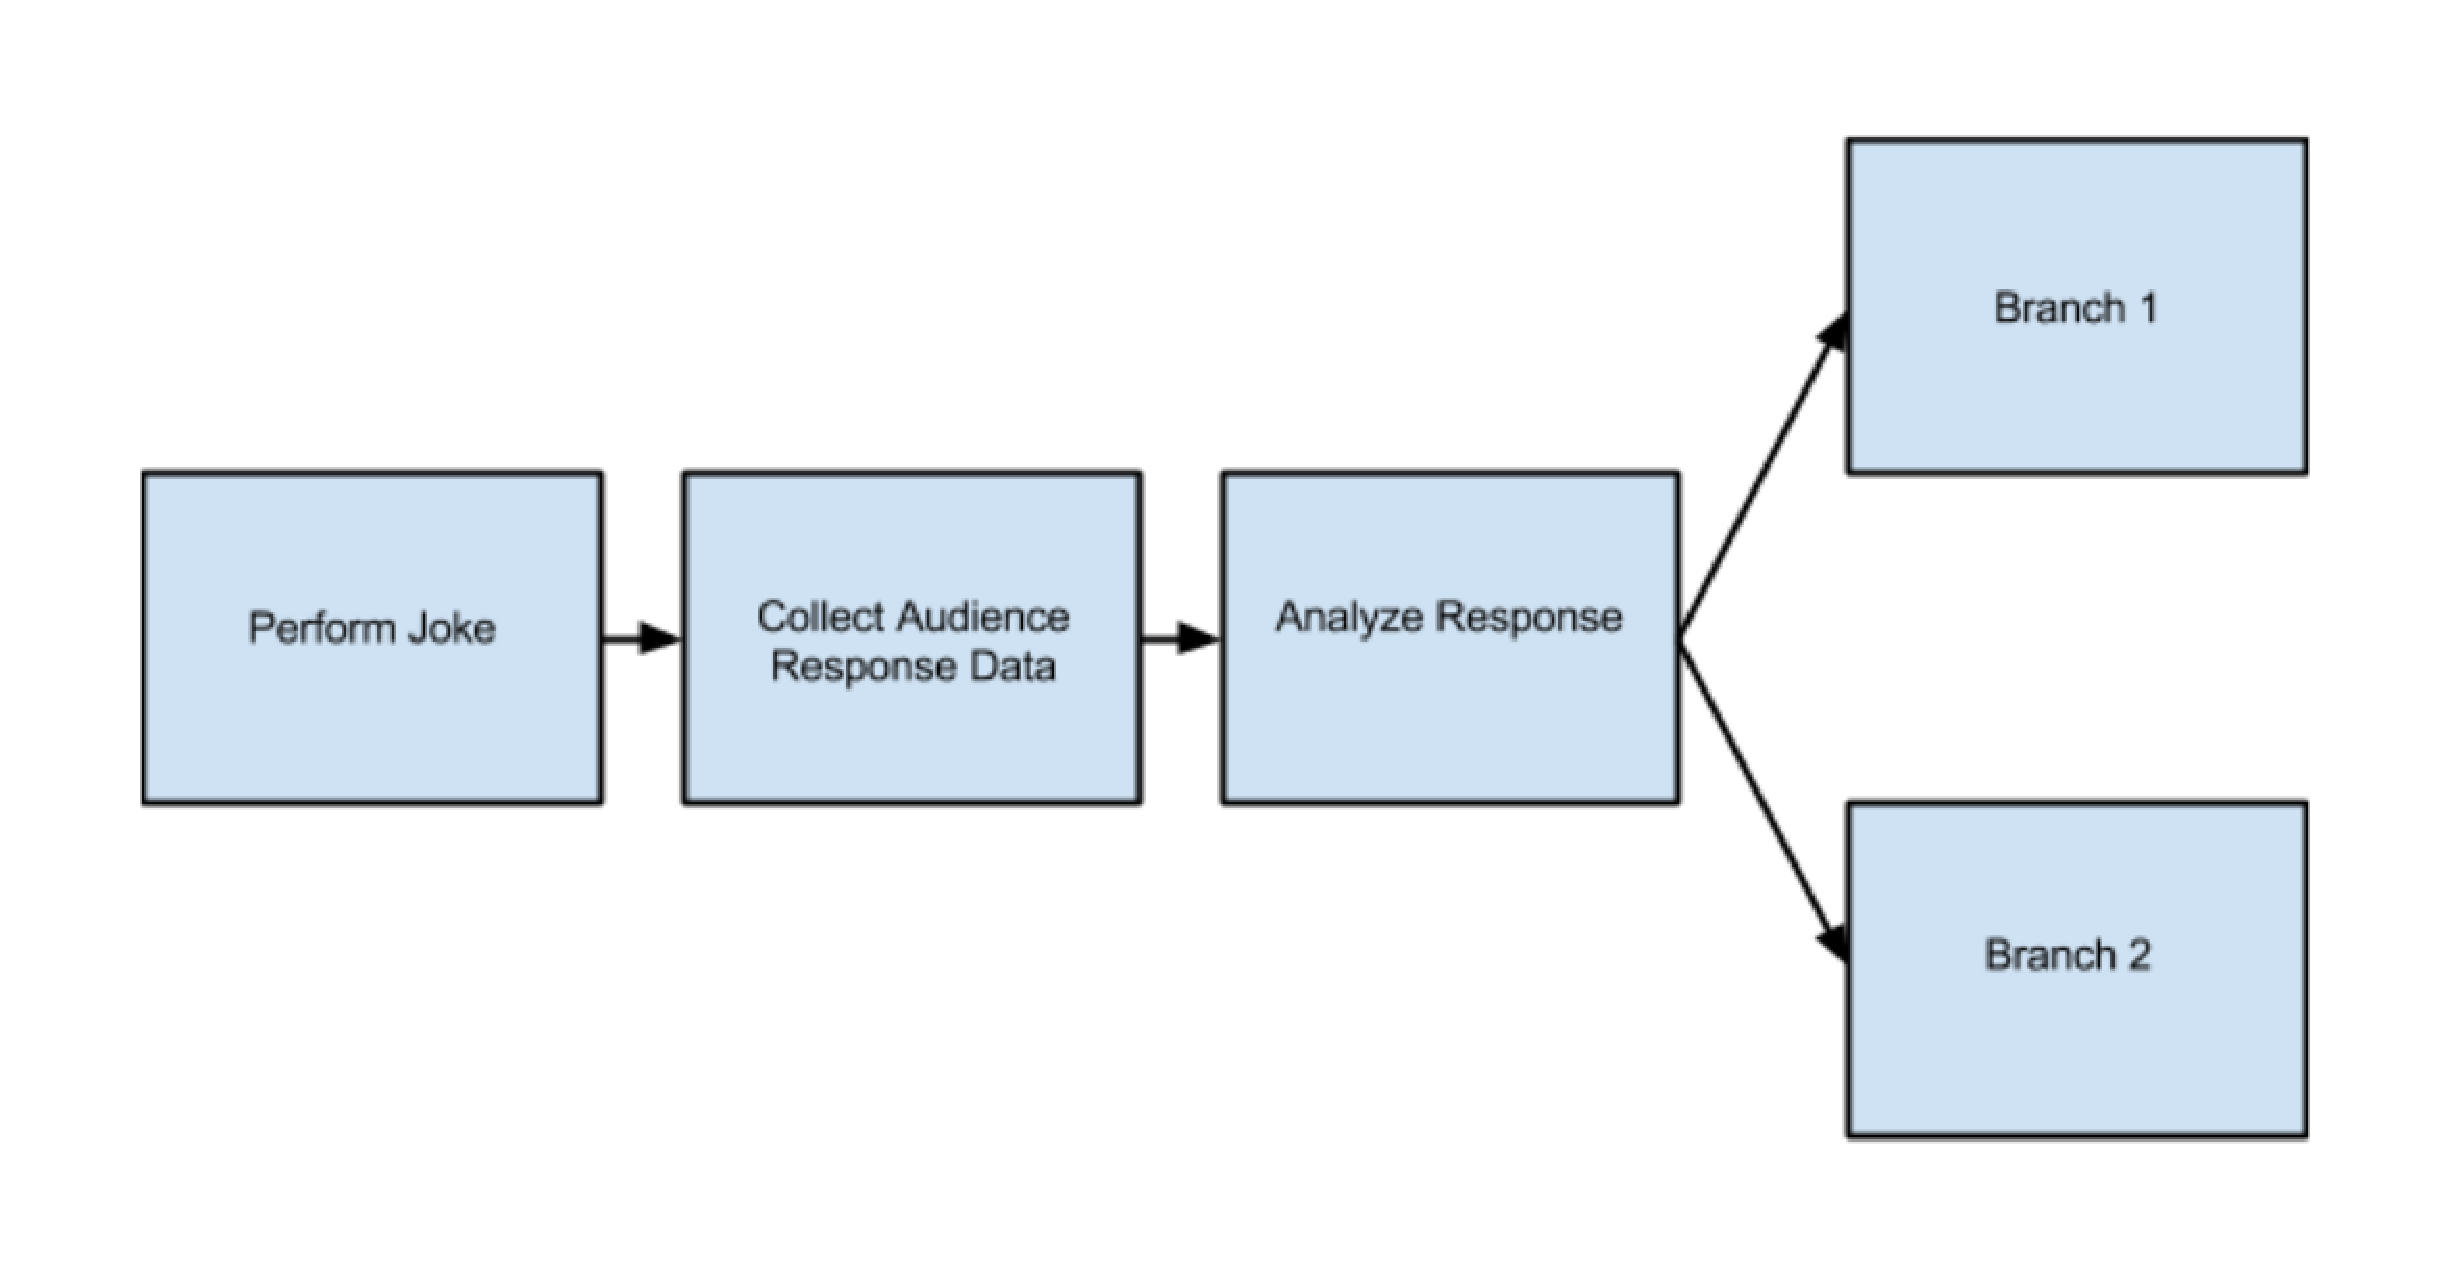
\includegraphics[width=0.75\textwidth,height=0.75\textheight,keepaspectratio]{fig1}
  \caption{ This flow-chart depicts how, once the robot delivers a joke, will wait for feedback, interpret data, and then make a joke decision (Branch 1 and Branch 2)}
  \label{fig:process}
\end{figure}

The close of the robot’s act will include the robot’s report of what attributes the audience
responded to most. The hypothesis here is that getting insight into the robot’s algorithms will increase the audience’s
perception of the robot’s intelligence, and, second, that it will make them laugh. People enjoy hearing about themselves.

All of the above behaviors, from adaptation to the end of performance audience report need to be evaluated with
real people. Initial tests will be done on campus with small groups of people, the final test will be done in conjuction
with the crowd-work and character manipulations, testing the entire algorithm together with a larger crowd, e.g., 10-25
people.


\subsection{Crowd-work}
\subsubsection{Goals}

Similar to the crowd report described above, we hypothesize that generally interacting with the audience (a.k.a crowd-
work) throughout the performance, will improve the audience’soverall enjoyment of the show. We want to analyze the

importance of this crowd-work relating to the central design of the project. Crowd-work should make the audience feel
like they are a part of the show. This can be done in different ways - calling out and talking to the audience, watching
the audience and incorporating them into the jokes, and asking them questions to keep them engaged, or to build off to
make new jokes.

\subsubsection{Methods}
There are various kinds of crowd-work we want to test: one research question is whether crowdwork matters at all, and
the second is does the crowdwork needs to be real or robot can just pretend it is paying attention?

To answer these questions we suggest three research conditions: (1) no crowdwork, (2) fake crowdwork, (3) real
crowdwork. The first one would be no crowd-work whatsoever. The robot goes about performing its set and does
not directly address the audience at all. The second could spanover-the-top and inaccurate crowd-work, or best-guess
crowdwork, with the possibility of being real (e.g., predicting that most people in the audience were from Oregon, even
if it didn’t really hear what they said). The third case would integrate actual robot sensing. It would be important for
conditions \#2 and \#3 to be parallel to assess whether crowdwork really matters.

As condition one is fairly obvious, let us discuss deeper possibilities for condition \#2. In the obviously fake research
condition, the robot will talk to the audience directly but it will be completely wrong in its observation. The absurdity
of a robot trying to understand the audience and being completely off could be entertaining for the audience, or it may
not connect with the audience at all. The exact reception of this sort of crowd-work is something we are trying to study.
The other version of condition \#2 is realistic but premeditated. For example, pre-known facts about the audience
could be built into the robot or guessed. These pre-known facts could include the location of the performance, age
demographics of the audience. For example, if the audience is known to be college-aged, the robot could be fed input
to make comments about things relevant to college students.

Using actual robot sensing data is condition \#3, and is certainly the ideal model, but requires sensing capabilities,
processing power and hardware, so it would be good to know if it is really necessary. In this condition, the robot would
be actually looking for cues from the audience during certain situations. For example, one example is asking questions
and capturing words from the audience, then using that same word later. For example, the robot could ask a simple
question about the weather, or the audience member’s hometown. In this case, the robot can listen for specific words
and ask another question about that specific town or city.

Another real sensing capability the robot could use is audience volume levels after the delivery of jokes. The robot
will keep track of the audience input. The robot could then acknowledge if the audience enjoyed the joke or did not
enjoy the joke using these inputs. Additional sensors and processing abilities on the Nao robot include face-detection
and bumper detection, so the exploration of audience sensing could potentially include speech, volume, vision, and
touch.

All of these condiditons will be assessed with live audiences (even if its just a few people in a classroom) to check to
what degree is crowd-work important for a robot comedian. The audience’s response will be used to see if they enjoy
a humanized robot or if they prefer a more robotic one, or maybe even a combination of both. As crowd work is just a
form of human interaction, we expect it will improve the audience’s perception of the robot’s intelligence, add surprise
to the show, and increase audience enjoyment levels. On the other hand, perhaps faking it can get 80% of the effect of
the real version. That will be part of the evaluation.



\subsection{Character}
\subsubsection{Goal}
The goal of this section of the project is to examine whether or not robot comedy can benefit from having jokes delivered
from a robot’s perspective. Our hypotheses are that a robot presenting jokes about technology or being a robot will be
funnier than a human telling the same jokes, and that robots will be less funny than humans at telling jokes from a
human perspective.

In Jerry Palmer's \textit{Taking Humor Seriously}, comic meaning is argued to depend on the interrelated factors of a joke's context and setting, its delivery, the identity of the deliverer, and the audience \cite{Palmer:1993}.
Of specific interest to us are the factors of a joke's delivery and the identity of the deliverer.
In previous studies, robot comedy has been used to analyze effective aspects of joke delivery.
However, little has been done in discovering effective aspects of a joke's content as it relates to the identity of the deliverer.
For example, Sj\"{o}bergh and Araki \cite{RobotsMakeThings:2008} found that jokes were perceived as funnier when delivered by a robot, rather than being delivered in text form.
However, Sj\"{o}bergh and Araki used word-play jokes that were gathered from the internet, and delivered them through a robot by using a flat, machine-like sounding text-to-speech tool called AquesTalk. This form of delivery does not take into account the importance of effective joke delivery. While Sj\"{o}bergh and Araki did not implement measures for analyzing non-verbal delivery, other work has examined the importance of non-verbal signals in delivering jokes \cite{KatevasRobot:2014} \cite{KnightEightLessons:2011}.
Despite this, there is little to no existing literature on the effectiveness of jokes related to the identity of the deliverer.
In our context, this means examining the effectiveness of robot-specific jokes in robot comedy.

\subsubsection{Methods}
To address this goal, jokes will be written from a human or robot perspective. The jokes written from a human
perspective will have a corresponding robot version, ideally with as much one-to-one correspondence as possible in
regards to cadence, length of joke, parrallel content, similar motions, and so forth. These jokes will be subject to intense
scrutiny by members of the project and by the client, such that revisions and edits can be made to create funny jokes
with a definite correspondence between the two versions. For example, a human version of a joke might look like the
following (lines with a definite correspondence with the robot version are highlighted):

\begin{lstlisting}
Hey, hey, I got news. This is big.
Ok, quiet down. Get this.
That's RIGHT folks.
I'm no longer single. *throws hands up*
(*@  \hl{I met a man on tinder.}  @*)
(*@  \hl{His name's Sebastian. He's a math nerd.}  @*)
(*@  \hl{Swiped right as fast as my fingers could move.}  @*)
\end{lstlisting}

Whereas, the robot version of the above joke is shown below.

\begin{lstlisting}
Hey, hey, I got news. This is big.
Ok, quiet down. Get this.
That's RIGHT folks.
I'm no longer single. *throws hands up*
(*@  \hl{I met a robot on tinder. }  @*)
(*@  \hl{His name's Data.  He's a really geeky robot.}  @*)
(*@  \hl{Swiped right as fast as my motors could turn.}  @*)
\end{lstlisting}

\subsubsection{Development process of joke writing}
These jokes will be scripted in Choregraphe, where adjustments to vocal tones and pausing will be made.
Then, animating the robot for non-verbal gestures will be done to enhance the delivery.
The overall process may look similar to Figure \ref{fig:write_process}.

\begin{figure}[H]
  \centering
  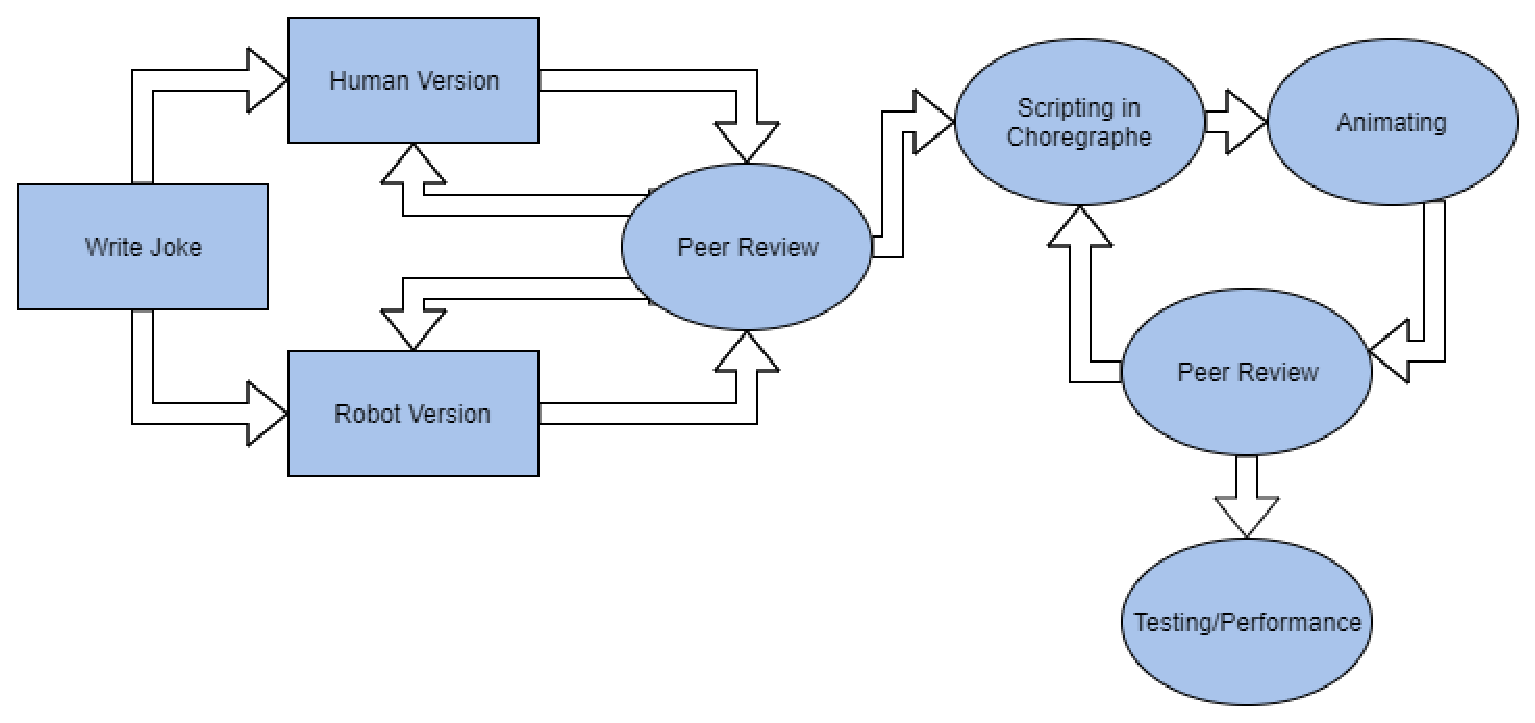
\includegraphics[width=0.75\textwidth,height=0.75\textheight,keepaspectratio]{joke_writing_process}
  \caption{The work flow from joke writing to testing.}
	\label{fig:write_process}
\end{figure}

\subsubsection{Experimentation}
The stand-up routine of the robot will comprise of text of the joke themselves, the motions that the robot uses to
accompany them, and the way the robot surveys the audience after each punchline, e.g., in a human or robotic fashion.
To determine the differences in audience response to the routines, studies will be done first on Amazon Mechanical
Turk, and later with co-located audiences. Participants will be shown a video of the robot’s stand-up routine, and then
presented with a short survey. The routines will be between 5 and 10 minutes long, and the survey will include questions
pertaining to each joke or routine. Participants will be compensated with standard rates for watching brief videos and
answering survey questions.

\section{Conclusion}
This document overviews our main Robot Comedy research questions, and the three software implementation targets
for the capstone: adaptation, crowd work, and robotic versus humanlike character. We hypothesize that all three will
play a role in designing an effective robot comedian.

Designs for the adaptive transitioning algorithm between jokes, the integration of an audience into the performance
of a set, and the exploration of robotic character in joke content and delivery have been described. To evaluate each,
we have described the hypotheses we have and the research conditions we will compare to validate or invalidate them.
People will be the ultimate judge of whether a robot performance will be successful, thus, human evaluations are critical.
This project will use of combination of in-person and video studies to evaluate each research question individually in
the winter term, then bring all parts of the programming together for collective evaluations with larger audiences on
campus in the spring.

In following through with this in the research and development process, we will better understand the role of
acknowleding and interacting with the audience, as well as the robot character itself, if creating experiences between
people and robots, on and off the stage. Not all robots will tell jokes, but understanding more about what people value
in robots could be reused in related robot applications from tour guides to english teachers, or even a factory robot that
delivers parts and lightens a worker’s day by making jokes about her favorite sports team.



\pagebreak

\pagebreak
\clearpage
\section{Glossary}
\begin{description}
  \item [Algorithm] \hfill \\ The software program that receives input to make an optimized choice; in this project, the algorithm is in context to the adaptation program.
	\item [Animating] \hfill \\ The NAO robot can be programmed to animate and move while speaking. This can be used to improve non-verbal communication between the robot and the audience.
  \item [API] \hfill \\ Application Programming Interface
  \item [Branch] \hfill \\Looking at the graph (edges and nodes) of a performance, a branch is a decision choice made by the algorithm.
  \item [Choregraphe] \hfill \\ Software used to program behavior and performance sets, made by SoftBank Robotics
  \item [Closing Joke] \hfill \\The final joke in a performance; this is helpful if it is a successful joke to end on a good note.
  \item [Crowd-work] \hfill \\ Part of a Comedian's performance that involves content from the current audience
  \item [NAO] \hfill \\ Model of Robot that will be used as the Comedian Agent, made by SoftBank Robotics
  \item [SoftBank Robotics] \hfill \\ Manufacturer of the NAO robot, NAOqi API, and Choregraphe software
  \item [Seed Jokes] \hfill \\ Set of three jokes that initialize the adaptation algorithm.
  \item [Set] \hfill \\Short for "Stand-up" set; this may also be used to describe to the collection of jokes: "A Set of Jokes"
  \item [Tree] \hfill \\This is the path through the set of jokes the algorithm took during a performance

\end{description}

\bibliographystyle{IEEEtran}
\bibliography{refs}

\end{document}
